\documentclass[a4paper,11pt]{article}
\usepackage[utf8]{inputenc}            % Tekenkodning
\usepackage[T1]{fontenc}               % Fixa kopiering av texten
\usepackage[english]{babel}            % Språk (t.ex. Innehåll)
\usepackage{geometry}                  % Sidlayout m.m.
\usepackage{graphicx,epstopdf,float}   % Bilder
\usepackage{amsmath,amssymb,amsfonts}  % Matematik
\usepackage{enumerate}                 % Fler typer av listor
\usepackage{fancyhdr}                  % Sidhuvud/sidfot
\usepackage{hyperref}                  % Hyperlänkar
\usepackage{parskip}                   % noindent!!
\usepackage{float}                     % \begin{figure}[H] preciserar bildposition
\usepackage{subcaption}             % För att lägga figurer bredvidvarandra från: http://tex.stackexchange.com/questions/91224/placing-two-figures-side-by-side
\usepackage{textcomp}
\usepackage{gensymb}
\usepackage{wrapfig}

% Add new commands used-defined:
\newcommand{\m}[1]{\mathbf{#1}}


% instälningar för figurtexter
\usepackage[margin=3ex,font=small,labelfont=bf,labelsep=endash]{caption}

% mailadresser som hyperlänkar
\newcommand{\mail}[1]{\href{mailto:#1}{\nolinkurl{#1}}}
% Spara författare och titel
\let\oldAuthor\author
\renewcommand{\author}[1]{\newcommand{\myAuthor}{#1}\oldAuthor{#1}}
\let\oldTitle\title
\renewcommand{\title}[1]{\newcommand{\myTitle}{#1}\oldTitle{#1}}

% Hyperlänkar
\hypersetup{
  colorlinks   = true, %Colours links instead of ugly boxes
  urlcolor     = black, %Colour for external hyperlinks
  linkcolor    = black, %Colour of internal links
  citecolor   = black %Colour of citations
}



\graphicspath{{./images/}} % Söker också bilder i en undermapp figs.


%% DOCUMENT
%------------------------------------------------------------------%
\begin{document}
  \title{Crack Detection using Inductive Methods}


  \author{
    Måns Bermell (\mail{mabe0395@student.umu.se})\\
    Joar Svartholm (\mail{josv0150@student.umu.se})
    }


  \date{\today}


\begin{titlepage}
  \maketitle
  \thispagestyle{fancy}
  \headheight 35pt
  \rhead{\small\today}
  \lhead{\small Department of Physics\\
    Umeå University}


% State the aim of the experiment, what was measured, which techniques and methods were used, and the main result(s) and conclusion(s). Remember that the abstract should be understandable on its own, and you can thereby not refer to equations/figures/tables in the report. You should also not use references, since the information in the abstract should be available in the actual report.
\vspace{1cm}
\begin{abstract}
\noindent
The Nobel prize in physics went in 2017 to the group who confirmed the prescence of gravitational waves. This was discovered using a type of Michelson interferometer sensing small changes in space. In this experiment, a Michelson interferometer was built in order to measure the refractive index of different gases. This could be done since light travels at different velocities in different materials. A change in refractive index, i.e. a change in pressure of a gas could be measured using this device with high accuracy. The refractive index of air was determined to 1.000264(6) which can be compared to the tabulated value of 1.000271. For argon, the index of refraction was calculated to 1.000253(9) and for nitrogen 1.000269(6). These values was also slightly below their tabulated values. This could be due to a systematic error in the calibration or an underestimation of the error. The refractive index of helium was calculated to 1.000034(4) which is higher that the tabulated value of 1.000032. The reason why the 


\end{abstract}

  % Ändra till rätt namn m.m.
  \cfoot{Non-invasive measurement techniques / v1.0\\
    Supervisor: Piotr Matyba }

\end{titlepage}


\newpage
\pagestyle{fancy}
\headheight 30pt
\rhead{\small \myTitle\\\today}
\lhead{\small \myAuthor}
\cfoot{\thepage}

% Innehåll
%\tableofcontents

%\newpage
\section{Introduction}

The 2017's Nobel price in physics was awarded to the group who confirmed Einstein's theory about gravitational waves. These waves was detected via an enormous interfermoeter. An interfermoeter can measure very small changes in optical paths and works by utilizing coherant light and the physical phenomena of interference. 

Light is the fastest moving thing know to humans, it travels at $299.792.458$ m/s in vaccum. This speed actually depends on the matter i travels in, for example, in water the speed is only $75\%$ compared to vaccum. These different speeds are inversly proportional to a materials index of refraction. 

In this report, the index of refraction is calculated for air, helium, argon and nitrogen. These were determined by examining the gases at different pressures in an Michelson interferometer.


\section{Theory}

\begin{equation}
  \label{eq:OPD}
  \tn{OPD} = 2\tn{OPL}_{L_2} - 2\tn{OPL}_{L_1} = 2nd + \tn{const.}
\end{equation}

where OPL is the optical path length

\begin{equation}
  \label{eq:interference}
  \tn{OPD} = N \lambda
\end{equation}

where $N$ is the number of interference fringes and $\lambda$ is the wavelength of the light. Putting this into Eq. \eqref{eq:OPD} yields

\begin{equation*}
  N \lambda = 2nd + \tn{const.}.
\end{equation*}

Instead of counting the absolute number of fringes one can count the number of fringes that appear when changing the refractive index of the sample, namely by increasing the pressure from vacuum then

\begin{equation*}
  \Delta N \lambda = 2d \Delta n = 2 d \alpha \frac{\Delta P}{P_0},
\end{equation*}

where $P$ is the absolute pressure,$P_0$ is the pressure according to STP conditions and $\alpha$ 




\section{Experimental setup}
% TODO: fixa röda tråden mellan metoden och utförandet.

The experimental setup used to measure the index of refraction for various gases is illustrated in Fig. \ref{fig:experimentalSetup}. The HeNe-laser beam is divided into two legs, reference leg $L_1$ and signal leg $L_2$ via a beam splitter (BS). The ray travelling down the signal leg is transmitted through a gas chamber made of acryllic glas, with inner length $d=100(1)$ mm. It is then reflected via a mirror back through the gas chamber and reflected on the beam splitter where it coincides with the other part of the ray (from the reference leg). The recombined laser beam propagates through a small apperature in order to eliminate unwanted reflections created by the equipment. The united ray also reaches a lens which diverge the rays in order to increase the resolution of the interference pattern obtained. A photodiode is mounted after the lens in order to pick up any changes of incident intensity of the combined laser beam. In order to eliminate ethalons inside the gas chamber, it was mounted at an angle relative to the incident laser beam.

\begin{figure}[H]
  \centering
  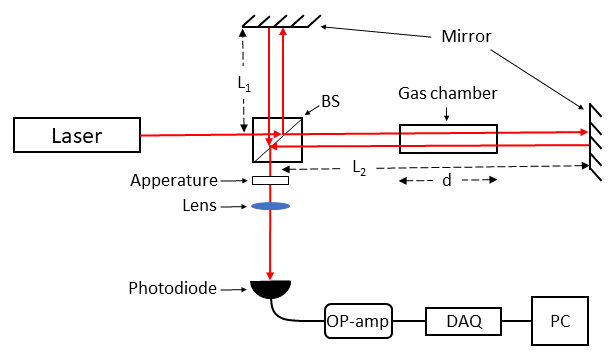
\includegraphics[width=0.8\textwidth]{Exp_setup.png}
  \caption{Experimental setup. BS is a beam splitter, $d$ is the width of the gas chamber, $L_1$ and $L_2$ are the lengths of the reference leg and the sensing leg respectively.}
  %\caption{Experimental setup. The laser beam is split into two rays at the beam splitter. One ray propagates in the reference leg (L$_1$) and is reflected back to the beam splitter. The other ray that was split at the beam splitter, propagates in to the signal leg (L$_2$) via a gas chamber to a mirror and reflected back the same way to the beam splitter. The two rays coincide at the beam splitter again and propagates through an apperature and a lens and illuminates a photodiode. The two rays will interfere with eachother and an interferance pattern will emerge.}
  \label{fig:experimentalSetup}
\end{figure}

The photodiode is connected to an operational amplifier with a low pass filter with a cut off frequency of 35Hz in order to amplify the signal and reduce noise in the circut. The data acquisition card (DAQ) retrives the amplified signal from the photodiode and a signal from a pressure sensor in the gas chamber.

The pressure signal was calibrated using a pressure gauge and the calibration curve is shown in Fig. \ref{fig:calibration}. A linear fit was done and the fitting parameters are found in Tab. \ref{tab:calibration}.
%The linear fit on the calibration measurement was calculated in by linear least squares in MATLAB, the fitted line has the equation $P = 12.5(2)V+25.6(1)$.

\begin{table}[H]
\centering
  \caption{Linear fit parameters $P = p_1 V + p_2$, for calibration of the pressure sensor.}
  \label{tab:calibration}
  \begin{tabular}{c|c|c}
    & $p_1$ & $p_2$ \\ \hline
    Pressure calibration & $12.5(2)$ kPa/V & $25.6(1)$ kPa
  \end{tabular}
\end{table}

\begin{figure}[H]
  \centering
  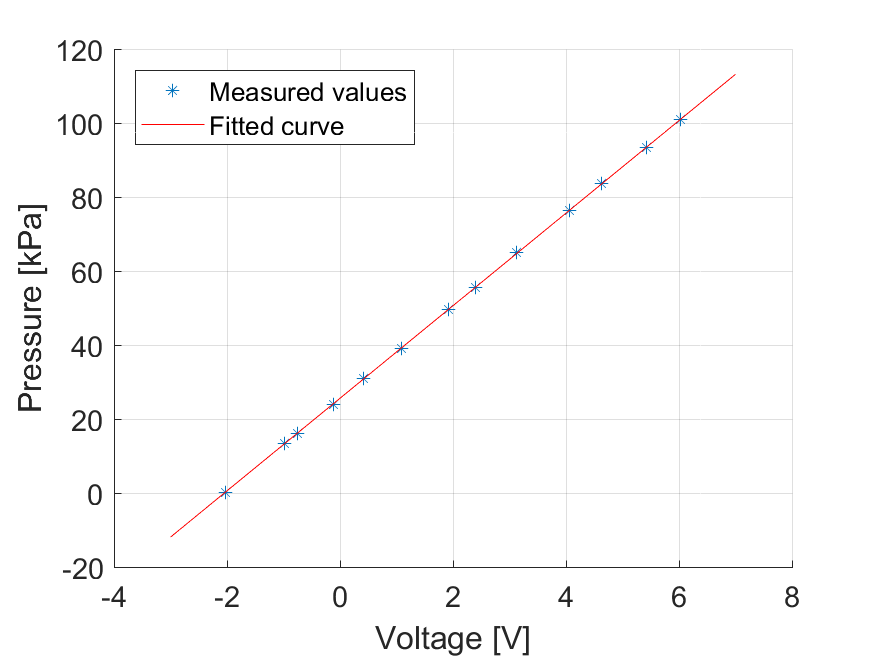
\includegraphics[width=0.8\textwidth]{matlab/calibration.png}
  \caption{Calibration curve for voltage to pressure relation. The linear fit parameters are found in Tab. \ref{tab:calibration}.}
  \label{fig:calibration}
\end{figure}

The two legs were aligned properly in order to see a interference pattern at the photodiode with high resolution and contrast. The gas chamber was filled with gas from vaccum and the intensity at the photodiode and the pressure in the gas chamber was measured continuously. Then by counting the fringes (intensity peaks at the photodiode) the index of refraction was calculated via Eq. \ref{eq:refrVaccum} and Eq. \ref{eq:slope}.

%, an interferance pattern will emerge on the photodiode. If vaccum is created inside the gas chamber and then a steady flow of gas added, the optical path will increase. An interferance pattern (fringes) on the photodiode  will start to move continuously. By measuring the intensity changes on the photodiode and relating this to the pressure change in the gas chamber, one can calculate the index of refraction via Eq. \ref{eq:refrVaccum} and Eq. \ref{eq:slope}.



In order to estimate the error of $a =\Delta N/ \Delta P$ from Eq. \ref{eq:slope}, the errors of $\Delta N$ and $\Delta P$ was estimated to $S_{\Delta N}=0.5$ and $S_{\Delta P}=0.1$ kPa. By fitting two lines that are inside these errors for all measurements, with as large slope/small slope as possible. These slopes will serve as the error estimates of $a$.


\section{Results and discussion}
The number of fringes was plotted against the pressure change for the different gases and is found in Fig. \ref{fig:measurements}. As one can see in the figures, all gases showed a linear relation which was expected according to the theory. When comparing Fig. \ref{fig:Helium} with the others, the number of fringes is a lot lower. This means that the index of refraction must be considerably lower for helium. It also implies that the relative error in the result will probably be larger in this result in comparison to the others.

The linear fit parameters are found in Tab. \ref{tab:linearFits}. As expected, the slope $a$ for helium is a lot lower than the other slopes. From these slopes, the refractive indexes was Calculated using Eq. \eqref{eq:slope} and tabulated in Tab. \ref{tab:refrIndex}.

\begin{figure}[H]
  \centering
  \begin{subfigure}{0.49\textwidth}
    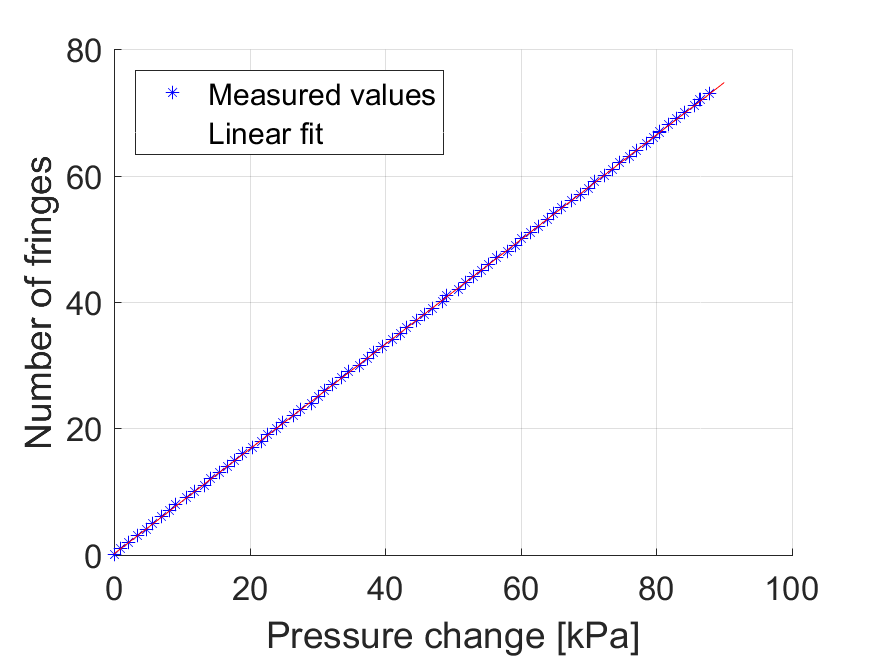
\includegraphics[width=\textwidth]{matlab/Air}
    \caption{Air}
    \label{fig:Air}
  \end{subfigure}
  \begin{subfigure}{0.49\textwidth}
    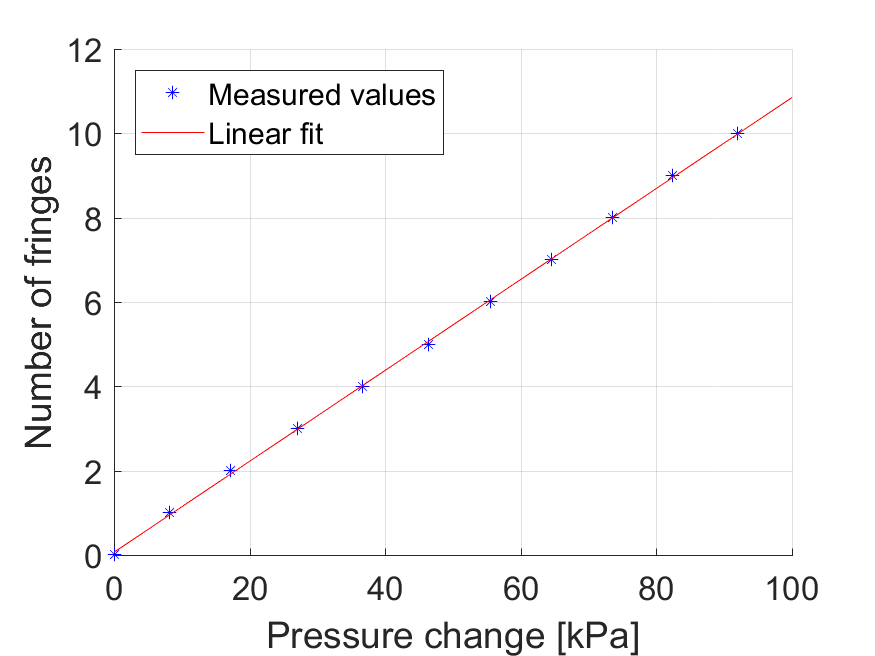
\includegraphics[width=\textwidth]{matlab/Helium}
    \caption{Helium}
    \label{fig:Helium}
  \end{subfigure}
  \begin{subfigure}{0.49\textwidth}
    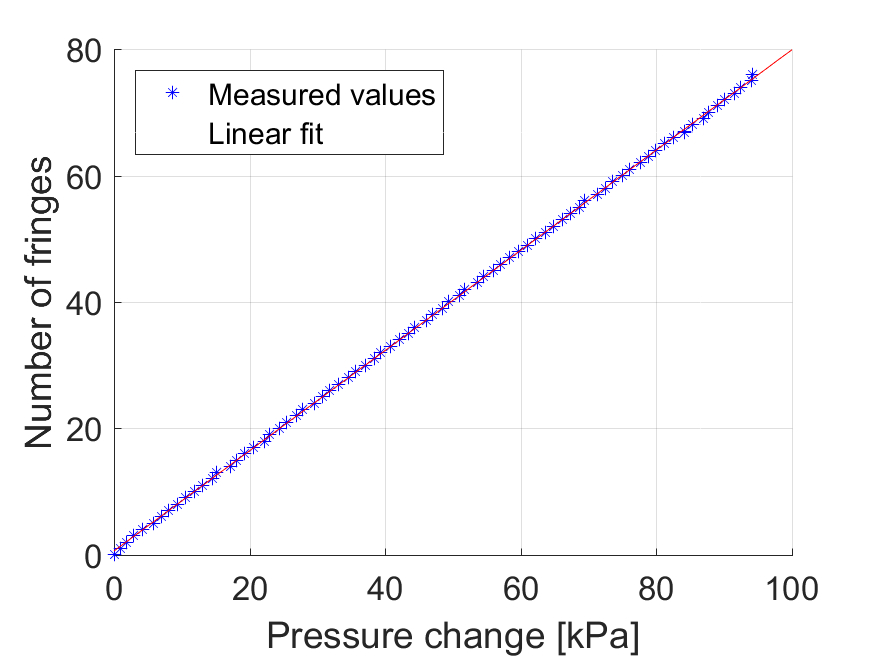
\includegraphics[width=\textwidth]{matlab/Argon}
    \caption{Argon}
    \label{fig:Argon}
  \end{subfigure}
  \begin{subfigure}{0.49\textwidth}
    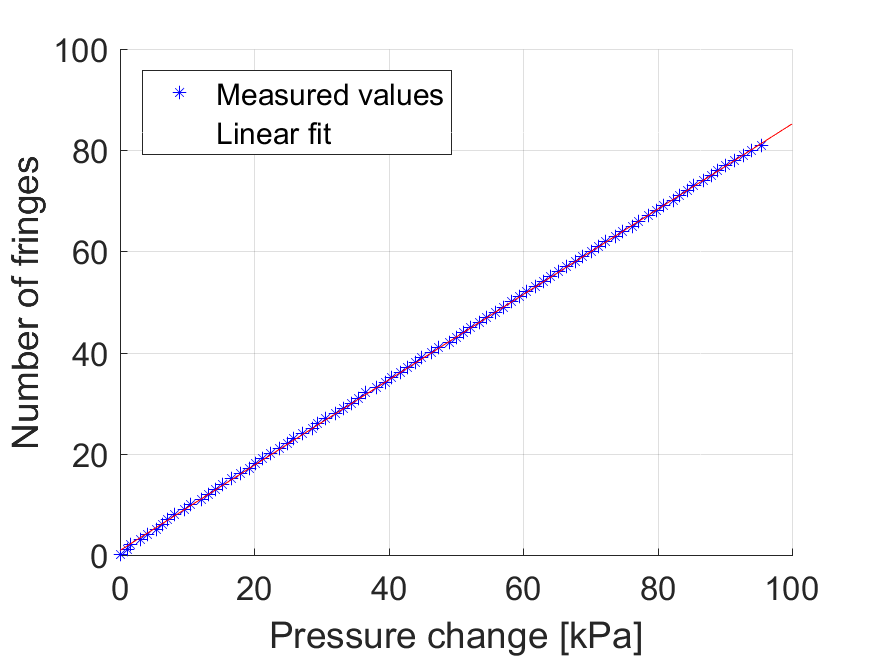
\includegraphics[width=\textwidth]{matlab/Nitrogen}
    \caption{Nitrogen}
    \label{fig:Nitrogen}
  \end{subfigure}
  \caption{Number of fringes and pressure change for the different gases with linear fits. Fitting parameters are found in Tab. \ref{tab:linearFits}}
  \label{fig:measurements}
\end{figure}

\begin{table}[H]
  \centering
  \caption{Fitting parameters for the measured values in Fig. \ref{fig:measurements}. Linear fit on the form $y=\alpha x + \beta$.}
  \label{tab:linearFits}
  \begin{tabular}{l|l|l}
           & $\alpha$ [kPa$^{-1}$]& $\beta$ \\ \hline
  Air      & $0.83(2)$  & $0.16(6)$ \\
  Helium   & $0.11(1)$ & $0.06(5)$ \\
  Argon    & $0.79(3)$ & $0.61(5)$ \\
  Nitrogen & $0.84(2)$ & $0.86(5)$
  \end{tabular}
\end{table}

\begin{table}[H]
  \centering
  \caption{Estimated refractive indexes for the gases including tabulated values \cite{idxAir}-\cite{idxNit}}
  \label{tab:refrIndex}
  \begin{tabular}{l|l|l}%|l}
          & Calculated & Tabulated  \\ \hline %& Error \\ \hline
    Air      & $1.000264(6)$  & $1.000271$  \\ %& $7.05654305 \cdot 10^{-6}$ \\
    Helium   & $1.000034(4)$  & $1.000032$  \\ %& $2.07707264 \cdot 10^{-6}$ \\
    Argon    & $1.000253(9)$  & $1.000261$  \\ %& $8.23800429 \cdot 10^{-6}$ \\
    Nitrogen & $1.000269(6)$  & $1.000276$  \\ %& $7.55338923 \cdot 10^{-6}$
  \end{tabular}
\end{table}

As seen in table \ref{tab:refrIndex} the tabulated values fo the refractive indexes are inside the error margin for helium and argon and slightly outside for air and nitrogen. Notice that the relative error is wastly larger for helium than for the others since it generated fewer fringers due to its smaller index of refractive. Note also that the calculated values are lower compared to the tabulated values for all gases but helium indicating that there might be a systematic error that is unknown. One reason for this could be that the measurements was not taken from perfect vaccum. The pump that was used to generate vaccum only achieved about 0.2-0.4kPa of pressure which intruduces a shift of the measurements. Since the refractive index at this pressure is still approximatly one in Eq. \ref{eq:refrInd}, only the right hand side would shift which would introduce a slightly higher slope $\alpha$. Then question then would be why the refracted index of helium was higher. This could be due to that the lack of measurements overtake this error in the opposite direction.

Another hypothesis of the systematic error is that the gas chamber contained a mix of different gases, most probably air since the pump device was unplugged between measuring the different gases. If the chamber had a combination of air and the other gas examined, it would result in a index of refraction slightly tilted towards the value for air. This theory would overestimate all index of refractions which are lower compared to air, as well as underestimating the ones with higher index of refraction. For our measuremnts this theory holds for helium and nitrogen. But does not explain the error relating to air index of refraction. The most trivial explination would be that we have underestimating the errors in the equipment used, which would make our estimated/calculated errors smaller than the true errors.


%All the tabulated values for index of refraction is within the calculated ones error of margin, as seen in Tab. \ref{tab:refrIndex}. The major thing to notice from the results is that the error margin for helium is approximatly five times larger than the errors for the other gases. This is expected, since helium generated only $10$ fringes while the other gases generated about $70-80$ fringes (i.e. alot more).


\section{Conclusion}



\begin{thebibliography}{}

\bibitem{phH} Nordling, C., \textit{Physics Handbook for Science and Engineering}, 2006

\bibitem{nP} Optics - Refractive index of air in dependence of temperature - Physics Stack Exchange. [ONLINE] Available at: \url{https://physics.stackexchange.com/questions/6872/refractive-index-of-air-in-dependence-of-temperature}. [Accessed 7 December 2017].

\bibitem{idxAir} Ciddor, P. E., \textit{Refractive index of air: new equations for the visible and near infrared}, Appl. Optics 35, 1566-1573 (1996)

\bibitem{idxHeli} Mansfield, C. R. and Peck, E. R., \textit{Dispersion of helium}, 1969.

\bibitem{idxArg} Bideau-Mehu, A., Guern, Y., Abjean, R., Johannin-Gilles, A., \textit{Measurement of refractive indices of neon, argon, krypton and xenon in the 253.7-140.4 nm wavelength range. Dispersion relations and estimated oscillator strengths of the resonance lines}, 1981.

\bibitem{idxNit} Peck, E. R. and Khanna, B. N., \textit{Dispersion of nitrogen}, 1966


\end{thebibliography}

%
% \include{appendix}



\end{document}
